\section{Model Selection and Assessment}
\textbf{Date:} \underline{Sep 9, 2025}

\subsection{Validation Sample}

\begin{figure*}[h]
    \centering
    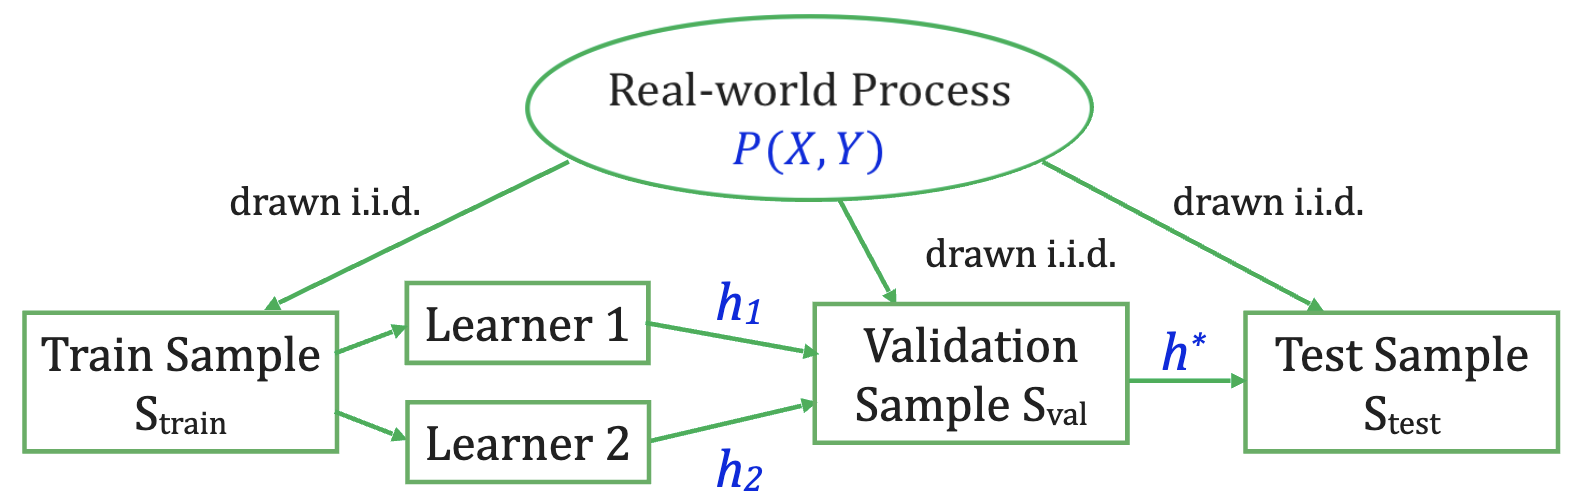
\includegraphics[width=0.8\textwidth]{Images/validation_sample.png}
    % \caption{Caption}
    % \label{fig:my_label}
\end{figure*}
\begin{itemize}
    \item \textbf{Training:} Run learning algorithm $l$ times (e.g. different parameters).
    \item \textbf{Validation Error:} Errors $err_{S_{val}}(h_i)$ are estimates of $err_{p}(h_i)$ for each $h_i$.
    \item \textbf{Selection:} Use $h^*$ with $\min\, err_{S_{val}}(\hat{h}_i)$ for prediction on test examples.
\end{itemize}

\paragraph{Two Nested Learning Algorithms}
\begin{itemize}
    \item \textbf{Primary Learning Algorithm on $S_{train}$}
    \begin{itemize}
        \item For each variant $A_1 \ldots A_l$ of learning algorithm, $h_i = A_i(S_{train})$
        \item Example: Decision Tree (DT) that stops at $i$ nodes.
    \end{itemize}
    \item \textbf{Secondary Learning Algorithm on $S_{val}$}
    \begin{itemize}
        \item Hypothesis space: $H' = \{h_1, \ldots, h_l\}$
        \item Learning Algorithm: $h^* = \arg\min\limits_{h \in H'} \left[ err_{S_{val}}(h) \right]$
    \end{itemize}
\end{itemize}

\paragraph{Typical ML Experiment}
\begin{itemize}
    \item Collect data $S = \left\{ \left( \vec{x}_1, y_1 \right), \ldots, \left( \vec{x}_m, y_m \right) \right\}$
    \item Split randomly into $S_{\text{train}}$, $S_{\text{val}}$, $S_{\text{test}}$
    \item REPEAT
    \begin{itemize}
        \item Train on $S_{\text{train}}$
        \item Validate on $S_{\text{val}}$
    \end{itemize}
    \item UNTIL we think we have a good rule $h$.
    \item Test $h$ on $S_{\text{test}}$ to evaluate its accuracy/error.
\end{itemize}

\subsection{Cross-Validation}
k-fold Cross-Validation:
\begin{itemize}
    \item \textbf{Given:}
    \begin{itemize}
        \item Training examples $S$
        \item Learning algorithm $A_p$ with parameter $p$ (model architectures or hyperparameters)
    \end{itemize}
    \item \textbf{Compute:}
    \begin{itemize}
        \item Randomly partition $S$ into $k$ equally sized subsets $S_1, \ldots, S_k$
        \item For each value of $p$:
        \begin{itemize}
            \item For $i$ from $1$ to $k$:
            \begin{itemize}
                \item Train $A_p$ on $S \setminus S_i$ and get $h_i$
                \item Apply $h_i$ to $S_i$ and compute $err_{S_i}(h_i)$
            \end{itemize}
            \item Compute cross-validation error:
            \[
                err_{CV}(A_p) = \frac{1}{k} \sum_i err_{S_i}(h_i)
            \]
        \end{itemize}
    \end{itemize}
    \item \textbf{Selection:}
    \begin{itemize}
        \item Pick parameter $p^*$ that minimizes $err_{CV}(A_p)$
        \item Train $A_{p^*}(S)$ on full sample $S$ to get final $h$
    \end{itemize}
\end{itemize}

\subsection{Generalization Error of Hypothesis}

\begin{itemize}
    \item \textbf{Given}
    \begin{itemize}
        \item Samples $S_{\text{train}}$ and $S_{\text{test}}$ of labeled instances
        \item Learning Algorithm $A$
    \end{itemize}
    \item \textbf{Setup}
    \begin{itemize}
        \item Train learning algorithm $A$ on $S_{\text{train}}$, result is $h$
        \item Apply $h$ to $S_{\text{test}}$ and compare predictions against true labels
    \end{itemize}
    \item \textbf{Test}
    \begin{itemize}
        \item Error on test sample $err_{S_{\text{test}}}(h)$ is estimate of true error $err_{p}(h)$
        \item Compute confidence interval
    \end{itemize}
\end{itemize}

\subsection{Significance Testing with the Binomial Distribution}

\begin{itemize}
    \item \textbf{Goal:} Assess whether the observed error rate of a hypothesis $h$ on a test set provides statistically significant evidence that the true error rate $err_P(h)$ is below (or above) a certain threshold.
    \item \textbf{Null Hypothesis:} Assume $err_P(h) \geq \epsilon$ for some threshold $\epsilon$.
    \item \textbf{Test Statistic:} Let $m$ be the number of test examples, and $k$ the number of observed errors. Under the null hypothesis, the number of errors $X$ follows a Binomial distribution: $X \sim \text{Binomial}(m, \epsilon)$.
    \item \textbf{p-value:} Compute the probability of observing $k$ or fewer errors under the null hypothesis:
    \[
        p\text{-value} = P(X \leq k \mid p = \epsilon, m)
    \]
    \item \textbf{Decision:} If the $p$-value is less than the significance level (e.g., $0.05$ for $95\%$ confidence), reject the null hypothesis and conclude that there is significant evidence that $err_P(h) < \epsilon$.
    \item \textbf{Interpretation:} This test quantifies how likely it is to observe the empirical error rate (or lower) if the true error rate were at least $\epsilon$.
\end{itemize}

\subsection{Normal Confidence Intervals}

\begin{itemize}
    \item \textbf{Rule of thumb:} When $mp(1-p) \geq 5$, the binomial distribution can be approximated by a normal distribution $N(\mu, \sigma^2)$ with $\mu = mp$ and $\sigma^2 = mp(1-p)$.
    \item \textbf{Normal confidence interval (95\% confidence):}
    \[
        err_P(h) \in \left[ err_S(h) - 1.96 \sqrt{\frac{p(1-p)}{m}},\; err_S(h) + 1.96 \sqrt{\frac{p(1-p)}{m}} \right]
    \]
    \item With approximation $p \approx err_S(h) \; \rightarrow$ Called ``Standard Error'' confidence intervals.
\end{itemize}

\subsection{Hoeffding Bound for Generalization Error}

\begin{itemize}
    \item \textbf{Hoeffding Bound:} For any loss function that takes values in $[0,1]$ and any hypothesis $h$, with probability at least $1 - \delta$ (where $1-\delta$ is called the \textbf{confidence level}), over the random choice of test samples $S$ of size $m$, the following holds:
    \[
        err_P(h) \in \left[ err_S(h) - \sqrt{\frac{-0.5 \ln(\delta/2)}{m}},\; err_S(h) + \sqrt{\frac{-0.5 \ln(\delta/2)}{m}} \right]
    \]
    \item This means that, with probability at least $1-\delta$, the true error $err_P(h)$ lies within the interval centered at the empirical error $err_S(h)$, with a margin that decreases as the number of test samples $m$ increases.
    \item The parameter $1-\delta$ is the probability that the interval contains the true error. For example, if $\delta = 0.05$, then $1-\delta = 0.95$ corresponds to a $95\%$ confidence interval.
\end{itemize}

\subsection{McNemar's Test}

\begin{itemize}
    \item \textbf{Given:}
    \begin{itemize}
        \item Two hypotheses $h_1$ and $h_2$
        \item Test set $S_{test}$ with $m$ examples
    \end{itemize}
    \item \textbf{Null Hypothesis:} $err_P(h_1) = err_P(h_2)$
    \begin{itemize}
        \item Implies that $err_S(h_1)$ and $err_S(h_2)$ come from binomial distributions with the same $p$
        \item Implies that the number of wins $w$ (where $h_1$ is correct and $h_2$ is not) and losses $l$ (where $h_2$ is correct and $h_1$ is not) follow:
        \[
            W \sim \text{Binomial}(p=0.5,\, n=w+l)
        \]
    \end{itemize}
    \item \textbf{Test:}
    \begin{itemize}
        \item Count wins $w$ and losses $l$ on $S_{test}$
        \item Reject the null hypothesis with $95\%$ confidence if:
        \[
            P(W \leq w \mid p=0.5,\, n=w+l) < 0.025
        \]
        or
        \[
            P(W \geq w \mid p=0.5,\, n=w+l) < 0.025
        \]
        \item \textbf{Why 0.025 instead of 0.05?} \\
        The total significance level is $0.05$ for a $95\%$ confidence test, but since McNemar's test is two-sided (we care if either $h_1$ is significantly better than $h_2$ or vice versa), we split the significance level equally between both tails of the distribution: $0.025$ for each tail.
    \end{itemize}
\end{itemize}